\question[10]
\mbox{}
\begin{center}
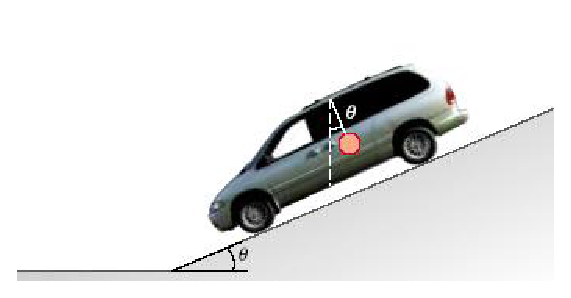
\includegraphics [scale=0.7]{./latex/eps/1_5_7_image_1.eps}
\end{center}
Mobil mengalami percepatan ketika menuruni bukit. Mobil awalnya diam kemudian mempunyai kecepatan 30 m/s dalam waktu 6 detik. Selama mobil dipercepat tergantung bandul (m= 0.1 Kg) pada atap mobil. Percepatan mobil sedemikian rupa sehingga bandul tetap tegak lurus atap mobil. Tentukan sudut $\theta$ dan tegangan tali? 

